Approaches to knowledge graph completion can be categorized according to various criteria, such as whether they operate on the pure graph or use auxiliary information, or whether they are primarily aimed at predicting facts or are designed for a downstream task. Furthermore, they can be grouped into symbolic and embedding-based approaches can be distinguished.

Symbolic approaches consider graphs in their ``natural'' form where entities and relations are distinguishable objects. The standard example of a symbolic approach is a rule miner that finds logical rules, which can then be used to predict new facts. The biggest advantage of symbolic approaches is that they process the symbols in a way that is comprehensible to humans, which also allows manually adding domain-specific knowledge. A limitation of distinct symbols is that similarities between them cannot be leveraged easily. For example, rules for the entity $City$ do not automatically apply to the entity $Town$. Another drawback can be poor scalability due to long computation times for large graphs.

In contrast to symbolic approaches are the embedding-based approaches that originate from the field of NLP where the concept is used to embed words in a continuous, low-dimensional vector space. Analogously, KGC models embed the entities and relations of a graph using floating-point vectors, which can be processed very efficiently by modern processors. Moreover, similarities between entities and relations can be covered. For example, the entity $City$ could be assigned a similar embedding as $Town$. Then, when processing $Town$-related knowledge, there is a good chance that patterns related to $City$ can be used. One disadvantage of embedded entities is that they must first be trained extensively until they reach their desired relative position to other embeddings, which may require large amounts of training data. Furthermore, the learned embeddings are not comprehensible to humans, making it harder to understand the model's decision.

Besides the pure facts of a knowledge graph, in practice, there is often additional information about the entities and relations such as textual descriptions that can be used in KGC. In particular, such additional information enables the support of open-world scenarios in which predictions shall be made for entities for which no facts exist are known.

In the following, \autoref{sec:3_related_work/1_symbolic} reviews symbolic approaches -- in particular the rule-based approach relevant to this work. Subsequently, \autoref{sec:3_related_work/2_embedding_based} gives an overview of different approaches of the widespread, state-of-the-art embedding-based models. Finally, \autoref{sec:3_related_work/3_additional_information} shows how embedding-based models incorporate additional information, such as textual entity descriptions, to improve performance before \autoref{ch:4_approach} continues to explain how the model uses additional information in combination with a rule-based model.


\section{Symbolic KGC}
\label{sec:3_related_work/1_symbolic}
The classical, symbolic approach to knowledge graph completion consists of capturing patterns in the graph structure in the form of logical rules. An example of a rule would be $(X, lives~in, Netherlands) <= (X, born~in, Amsterdam)$, which states that a person born in Amsterdam lives in the Netherlands. Rules do not express absolute truths but are associated with confidences that indicate how reliable they are. For reasons of computability and runtime complexity, many rule miners restrict themselves to finding Horn rules. Although Horn rules cannot express any logical pattern, they are sufficient in practice.

The concept of logical rules is not new and has been used in inductive logic programming (ILP)~\cite{Muggleton1994InductiveLP}, such as ALEPH~\cite{ALEPH}, for a long time. However, ILP approaches do not scale very well with the size of modern knowledge graphs and mostly require negative examples, which are not given under the open-world assumption. This is addressed by modern approaches such as the \emph{top-down} rule miner AMIE~\cite{Galrraga2013AMIEAR} and its successor AMIE+~\cite{Galrraga2015FastRM} or the \emph{bottom-up} rule miner AnyBURL~\cite{Meilicke2019AnytimeBR}, which is used in this work. Thereby, top-down algorithms start their search for rules with general rules they try to find evidence for, while bottom-up approaches start with concrete paths in the graph which they try to generalize to rules.

Another way to find rules is \emph{differentiable rule mining}, implemented by neural theorem provers (NTPs)~\cite{Rocktschel2017EndtoendDP}, DRUM~\cite{Sadeghian2019DRUMED} and Neural LP~\cite{Yang2017DifferentiableLO}. These models represent rules numerically and thus enable end-to-end learning of rules. To represent a rule numerically, they encode a rule's facts as $|E| \times |E|$ matrices, that state which head entity $head \in E$ is connected to which tail entity $tail \in E$ by setting a $1$ in the matrix' respective cell. A rule is then represented by the $|E| \times |E|$ matrix calculated as the product of its facts' matrices. A limitation of the listed models is that they can only represent path-like rules.

An alternative symbolic approach to rule mining is the usage of \emph{description logics (DLs)}~\cite{Baader2003TheDL} to form so-called \emph{axioms} that capture patterns in the graph, which also have the advantage of being understandable to humans. An example of an axiom would be $Belgian \sqsubseteq DutchSpeaker \sqcup FrenchSpeaker$. As one can guess from the similarity to set operators, the axiom states that Belgians speak either Dutch, French, or both. Just like rules, those axioms are not inherently true but hold with a certain confidence. The mentioned axiom, for example, does not consider German-speaking Belgians. Two concrete axiom miners are the ones created by Völker et al.~\cite{Vlker2015AutomaticAO} and Töpper et al.~\cite{Tpper2012DBpediaOE}.



\section{Embedding-Based KGC}
\label{sec:3_related_work/2_embedding_based}
Most of the current, state-of-the-art knowledge graph completion models are based on the idea that the objects of interest can be embedded as low-dimensional, numerical vectors that can be computed effectively and efficiently by downstream models as proven in multiple other fields in the recent past, such as NLP and image processing~\cite{Wang2017KnowledgeGE}. Thereby, low-dimensional referrs to vectors limitted to a few hundred dimensions, which is low compared to comparable one-hot encodings. Equivalent to words in NLP and images in image processing, the embedded objects in KGC are a knowledge graph's entities and relations, although in practice many KGC models merely embed a graph's entities directly, while the relations' embeddings are implied, for example by the entities' relative positions to each other.

The overall process by which meaningful embeddings are created often starts with randomly initializing entity embeddings - and relation embeddings if they are represented explicitly. During training, a KGC model then repeatedly calculates the probability of facts using a scoring function that takes a fact's entity and relation embeddings as input. Thereby, the training objective is to rearrange the entity and relation embeddings so that the scoring function produces high probabilites for true facts and low probabilites for wrong facts. That rearrangement is performed by minimizing a loss function, that could be the negative of the scoring function, using backpropagation. Although most approaches see the graph under the open-world assumption, many support training by producing false facts artificially, known as \emph{negative sampling}, by corrupting true facts, i.e. replacing a true facts head or tail entity with another, random entity. Thereby, chances are high to generate a truly false fact that helps with discriminating true and false facts. At the end of training, the knowledge graph is embedded in a way that captures the structure of the original graph and can be used for further reasoning via cheap vector operations.

Various KGC models differ in their choice of a concrete embedding space, whether and how they embed relations as well as the kind of scoring function they use. As for the embedding space, many models embed the graph in a real-valued, euclidean space, whereas other models chose complex or non-euclidean spaces. Concerning relations, some models embed them implicitly as the relative position between entity embeddings, while others assign vectors, matrices or even tensors to each relation. Finally, models differ in whether they use a distance-based or a similarity-based scoring function. Overall, embedding-based KGC models can be roughly grouped into translational, tensor decomposition, neural and language models.

\begin{figure}[t]
    \centering
    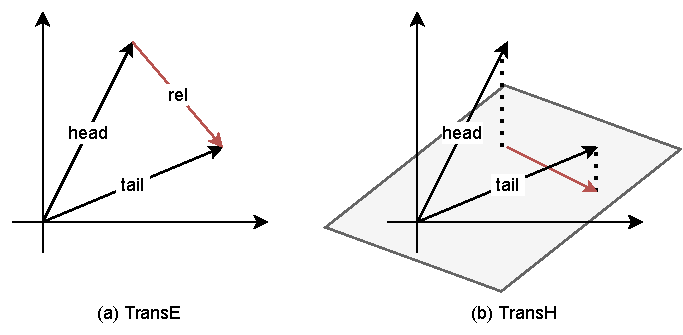
\includegraphics{3_related_work/2_embedding_based/translational}
    \caption{Concept behind translational KGC models: Relations are implicitly represented as vectors between entities - either (a) directly, as for TransE, or (b) indirectly, as for TransH, which projects entity embeddings to relation-specific hyperplanes before performing translation, which supports more complex relations.}
    \label{fig:3_related_work/2_embedding_based/translational}
\end{figure}

From the different kind of models, translational models might be the most intuitive ones. The first and simplest one is TransE~\cite{Bordes2013TranslatingEF} whose basic idea is similar to the concept behind the language model word2vec~\cite{Mikolov2013EfficientEO}: Just like the latter embeds words such that differences between word embeddings reflect semantic relations, TransE embeds entities so that differences between entity embeddings imply relations between them. For example, in word2vec the vector between the word embeddings "king" and "man" is similar to the vector between "queen" and "woman". Analogously, in the embedding space learned by TransE, one might get from the entity embedding of "king" to the entity embedding of "man" by adding the embedding of the relation "is royal" to the entity "king". Figure~\ref{fig:3_related_work/2_embedding_based/translational} illustrates the concept. Formally, given a fact $(\textbf{head}, \textbf{rel}, \textbf{tail})$, TransE learns embeddings such that $\textbf{head} + \textbf{rel} \approx \textbf{tail}$ if the fact is true and $\textbf{head} + \textbf{rel} \neq \textbf{tail}$ if not. It thus minimizes a loss function that aims at maximizing the score function, which is the negative distance between the predicted and the actual tail embedding:

\begin{align}
    score(\textbf{head}, \textbf{rel}, \textbf{tail}) = {- || \textbf{head} + \textbf{rel} - \textbf{tail} ||}_{2}
    \label{eq:3_related_work/2_embedding_based/trans_e}
\end{align}

Problems with TransE's simple approach arise when it comes to 1-n, n-1 and n-m relations. For example, representing the facts $(Ed, speaks, Dutch)$ as well as $(John, speaks, Dutch)$ would require the entities of Ed and John to be roughly at the same spot in embedding space, but other relations between the two might require them to be apart from each other. Also problematic are cyclic relations, such as "married to", because TransE learns that all relations are represented by a vector of zeros. This is where other translational models step in. TransH~\cite{Wang2014KnowledgeGE}, for example, maps the entities onto relation-specific hyperplanes as illustrated in Figure~\ref{fig:3_related_work/2_embedding_based/translationa} before performing the translation. That way multiple entities can be projected onto the same spot on the hyperplane without being at the same location in space. Similarly, TransR~\cite{Lin2015LearningEA} maps entity embeddings into separate, relation-specific embedding spaces, while other models like RotatE~\cite{Sun2019RotatEKG} and MuPR~\cite{Balazevic2019MultirelationalPG} take another approach and work in complex or hyperbolic embedding spaces, which provide "enough room" for the respective relations.

\begin{figure}[t]
    \centering
    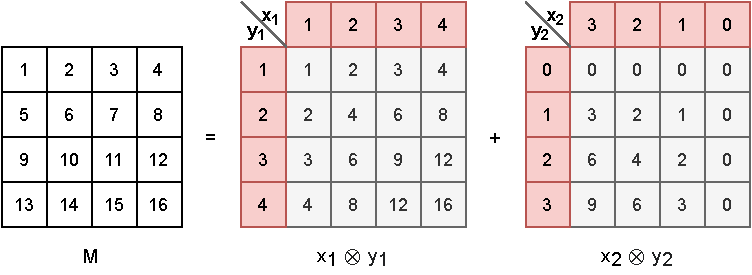
\includegraphics{3_related_work/2_embedding_based/tensor_decomposition}
    \caption{Example for tensor decomposition: A high-dimensional tensor (here, the matrix $M$) can be approximated as the sum of outer products of lower-dimensional tensors (here, the vectors $x_1$, $y_1$, $x_2$ and $y_2$).}
    \label{fig:3_related_work/2_embedding_based/tensor_decomposition}
\end{figure}

Different from translational KGC models, tensor decomposition models are based on the idea that the graph embedding space can be expressed as a composition of many smaller tensors that represent entities and relations. Figure~\ref{fig:3_related_work/2_embedding_based/tensor_decomposition} demonstrates tensor decomposition by an example: A matrix, which is a two-dimensional tensor, can be calculated as the sum of two outer vector products between four vecctors, which are one-dimensional tensors. Likewise, a graph $G$ can be approximated by $3 \times d$ d-dimensional vectors:

\begin{align}
    G \approx \sum_{i=1}^{d} \textbf{x}_i \otimes \textbf{y}_i \otimes \textbf{z}_i
    \label{eq:3_related_work/2_embedding_based/tensor_decomposition}
\end{align}

The mathematics behind tensor decomposition can then be used to optimize the similarity-based scoring function of tensor decomposition models. For example, Equation~\ref{eq:3_related_work/2_embedding_based/distmult} shows the score function of DistMult~\cite{Yang2015EmbeddingEA}, which corresponds to optimizing a tensor decomposition where entities and relations are represented by d-dimensional vectors.

\begin{align}
    score(\textbf{head}, \textbf{rel}, \textbf{tail}) = \sum_{i=1}^{d} \textbf{head}_i \cdot \textbf{rel}_i \cdot \textbf{tail}_i
    \label{eq:3_related_work/2_embedding_based/distmult}
\end{align}

Again, the goal of training is to find embeddings that maximize the scoring function for true facts and minimize it for false facts. Thereby, one limitation of DistMult is that its relation vectors cannot capture asymmetric relations. Other models follow different attempts to solve this problem. For example, RESCAL~\cite{Nickel2013TensorFF} represents relations using matrices instead of vectors, HolE~\cite{Nickel2016HolographicEO} leverages the non-comulativity of the correlation operators, ComplEx~\cite{Trouillon2016ComplexEF} works in complex space, and TuckER~\cite{Balazevic2019TuckERTF} employs Tucker decomposition.

\begin{figure}[t]
    \centering
    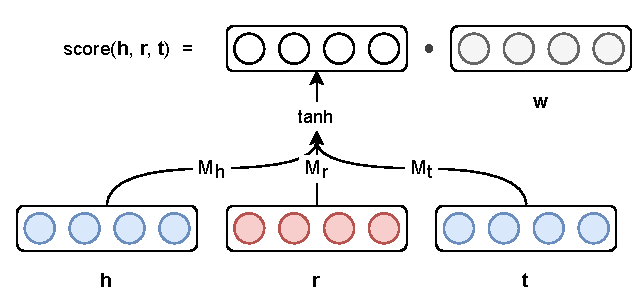
\includegraphics{3_related_work/2_embedding_based/mlp}
    \caption{Architecture of the neural MLP model~\cite{Dong2014KnowledgeVA}. In the first layer, a fact $(\textbf{h}, \textbf{r}, \textbf{t})$ is embedded using three matrices for head, relation and tail embeddings as well as the non-linear $\tanh$ function. In the second layer, the fact's score is calculated as the scalar product of the fact embedding and a weight vector $w$.}
    \label{fig:3_related_work/2_embedding_based/mlp}
\end{figure}

Yet nother approach towards KGC is followed by neural models like MLP~\cite{Dong2014KnowledgeVA} that leverage a non-linear function in a neural net to capture complex relations. Figure~\ref{fig:3_related_work/2_embedding_based/mlp} depicts the two-layer architecture of the MLP model. At the first layer, it multiplies entity and relation vectors with three matrices it keeps for head entities, relations and tail entities before it applies the non-linear $\tanh$ activation function to the sum of resulting vectors. In the second layers follows a simple scalar multiplication with a weight vectors, yielding the final score function:

\begin{align}
    score_{MLP}(\textbf{h}, \textbf{r}, \textbf{t}) = \langle tanh(M_h \cdot \textbf{h} + M_r \cdot \textbf{r} + M_t \cdot \textbf{t}), \textbf{w} \rangle
    \label{eq:3_related_work/2_embedding_based/mlp}
\end{align}

Similar approaches include SME~\cite{Glorot2013ASM}, one of the first models to use a neural network, NTN~\cite{Socher2013ReasoningWN}, which uses relation-wise tensors before applying the non-linear function, and NAM~\cite{LIU2016ProbabilisticRV}, which employs more layers in its deep architecture.

Finally, there are KGC approaches that use the achievements of NLP models even more than tranlsational ones like TransE, in that they directly employ language models. The idea is that the variable-length sentences, consisting of words, that a language model expects as input can be replaced with variable-length paths randomly sampled from the graph, whose path segments correspond to words. Two implementations from this category include RDF2Vec~\cite{Ristoski2016RDF2VecRG}, that builds upon the word2vec~\cite{Mikolov2013EfficientEO} language model, and KGloVE~\cite{Cochez2017GlobalRV}, which is based on GloVE~\cite{Pennington2014GloveGV}.



\section{Using Additional Information}
\label{sec:3_related_work/3_additional_information}
The symbolic and embedding-based approaches discussed so far purely rely on a knowledge graph's fact for prediction. This section presents models that leverage additional information, such as type information, textual entity descriptions or logical rules to improve predictions.

Type information is provided by some knowledge graphs to distinguish between different kinds of entities. A graph representing a social network, for example, might label entities as persons, locations or events. A simple model that leverages such type information is SSE~\cite{Guo2015SemanticallySK}, which keeps entities of the same type closer together during training. One of its drawbacks, however, is that it can only handle non-hierarchical types. In contrast TKRL~\cite{Xie2016RepresentationLO} extends on this and support hierarchical types as well as multiple type labels per entity. Another advantage of typed knowledge graphs is that types can be used to improve negative sampling: By excluding augmented negative samples with correct typings it can be guaranteed that no true facts are generated.

Another kind of additional information, and arguably the most comprehensive one, is textual entity descriptions. Dictionaries and encyclopedias contain concise definitions and descriptions for a wide range of entities and web crawlers can collect texts from vast online sources. The NTN~\cite{Socher2013ReasoningWN} model mentioned before was one of the first KGC models to leverage that information to initialize its entity embeddings by averaging the word embeddings of the entities' names. Similarly Long et al. used longer text descriptions to initialize entity embeddings~\cite{Long2016LeveragingLR}. However, both approaches have in common that the texts are not used to improve fact embeddings during training.

One of the earliest approaches to use texts beyond entity initialization was proposed by Wang et al~\cite{Wang2014KnowledgeGE}. who implemented joint embedding of facts and texts. Later, DKRL~\cite{Xie2016RepresentationLO}, an extension to TransE, and OWE~\cite{Shah2019AnOE}, an extension to embedding-based KGC models in genearl, have been developed. Both have the advantage that they can also be applied to open-world entities that are not seen during training. Figure~\ref{fig:3_related_work/3_additional_information/owe} illustrates the working of OWE: First, word embedding and graph embedding models are trained individually on the text and graph data. Then, an alignment function is learned that maps word embeddings to their respective entity embeddings. This allows texts of open-world entities to be mapped to the right position in the graph embedding space. In the example in Figure~\ref{fig:3_related_work/3_additional_information/owe} it would thus be possible to predict similar facts for the open-world entity John as for the known entity Ed it is close to.

\begin{figure}[t]
    \centering
    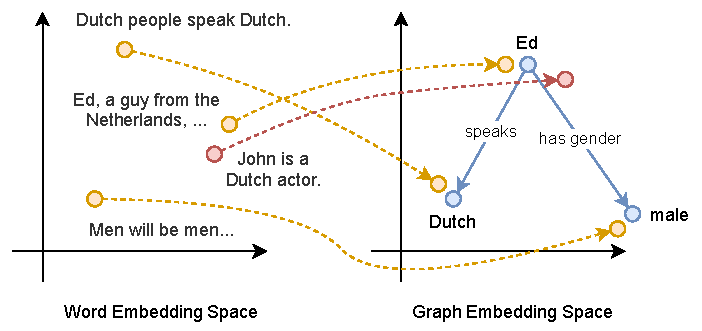
\includegraphics{3_related_work/3_additional_information/owe}
    \caption{The OWE model~\cite{Shah2019AnOE} learns a mapping function to align its separately learned word and graph embedding spaces, which allows predictions for open-world entities. Here, the text of the open-world entity John (red) is embedded close to the text of the known entity Ed, leading to similar embeddings in the graph embedding space, allowing OWE to predict similar facts for John.}
    \label{fig:3_related_work/3_additional_information/owe}
\end{figure}

Finally, beyond type and text information, some models also attempted to incorporate rules into training of embedding-based models. Some early approaches~\cite{Wang2015KnowledgeBC, Wei2015LargescaleKB} used them to put constraint on their predicted facts, but such a post-processing step does not help with training the actual graph embedding. The KALE model~\cite{Guo2016JointlyEK} on the other hand represents facts and rules in a common vector space. The basic idea is to ground the rules and calculate the rule groundings' embeddings from the facts they consist of using fuzzy logics. The probability of a fact $(h, r, t)$ is thereby based on the Manhatten distance between the $d$-dimensional vectors $h + r$ and $t$ as per Equation~\cite{eq:3_related_work/3_additional_information/kale_fac}, while Equation~\ref{eq:3_related_work/3_additional_information/kale_rule} gives an example of how the probability of a rule grounding with two body facts $f_1$ and $f_2$ and a head fact $f_3$ is calculated.

\begin{align}
    I(\textbf{h}, \textbf{r}, \textbf{t}) &= 1 - \frac{1}{3 \sqrt {d}} {|| \textbf{h} + \textbf{r} - \textbf{t} ||}_1
    \label{eq:3_related_work/3_additional_information/kale_fact} \\
    I(f_1 \land f_2 \Rightarrow f_3) &= I(f_1) \cdot I(f_2) \cdot I(f_3) - I(f_1) \cdot I(f_2) + 1
    \label{eq:3_related_work/3_additional_information/kale_rule}
\end{align}

Beyond Horn rules, KALE can handle any propositional logic rules. Given the formula for calculating an arbitrary rule's probability, which includes single facts, KALE then employs a margin-based ranking loss to learn the common embedding space that allows looking up ground path rules that are similar to facts and vice versa. The only drawback is that KALE cannot handle quantifiers from first order logic, which is why it uses rule groundings.

